%%%%%%%%%%%%%%%%%%%%%%%%%%%%%%%%%%%%%%%%%
% Tufte-Style Book (Minimal Template)
% LaTeX Template
% Version 1.0 (5/1/13)
%
% This template has been downloaded from:
% http://www.LaTeXTemplates.com
%
% License:
% CC BY-NC-SA 3.0 (http://creativecommons.org/licenses/by-nc-sa/3.0/)
%
% IMPORTANT NOTE:
% In addition to running BibTeX to compile the reference list from the .bib
% file, you will need to run MakeIndex to compile the index at the end of the
% document.
%
%%%%%%%%%%%%%%%%%%%%%%%%%%%%%%%%%%%%%%%%%

%----------------------------------------------------------------------------------------
%	PACKAGES AND OTHER DOCUMENT CONFIGURATIONS
%----------------------------------------------------------------------------------------

\documentclass[nobib]{tufte-book} % Use the tufte-book class which in turn uses the tufte-common class

\usepackage{natbib}
\setcitestyle{authoryear}
\bibliographystyle{plainnat}

\hypersetup{colorlinks} % Comment this line if you don't wish to have colored links

\usepackage{microtype} % Improves character and word spacing

\usepackage{lipsum} % Inserts dummy text

\usepackage{booktabs} % Better horizontal rules in tables

\usepackage{graphicx} % Needed to insert images into the document
\graphicspath{{graphics/}} % Sets the default location of pictures
\setkeys{Gin}{width=\linewidth,totalheight=\textheight,keepaspectratio} % Improves figure scaling

\usepackage{fancyvrb} % Allows customization of verbatim environments
\fvset{fontsize=\normalsize} % The font size of all verbatim text can be changed here

\newcommand{\hangp}[1]{\makebox[0pt][r]{(}#1\makebox[0pt][l]{)}} % New command to create parentheses around text in tables which take up no horizontal space - this improves column spacing
\newcommand{\hangstar}{\makebox[0pt][l]{*}} % New command to create asterisks in tables which take up no horizontal space - this improves column spacing

\usepackage{xspace} % Used for printing a trailing space better than using a tilde (~) using the \xspace command

\newcommand{\monthyear}{\ifcase\month\or January\or February\or March\or April\or May\or June\or July\or August\or September\or October\or November\or December\fi\space\number\year} % A command to print the current month and year

\newcommand{\openepigraph}[2]{ % This block sets up a command for printing an epigraph with 2 arguments - the quote and the author
\begin{fullwidth}
\sffamily\large
\begin{doublespace}
\noindent\allcaps{#1}\\ % The quote
\noindent\allcaps{#2} % The author
\end{doublespace}
\end{fullwidth}
}

\newcommand{\blankpage}{\newpage\hbox{}\thispagestyle{empty}\newpage} % Command to insert a blank page

\usepackage{makeidx} % Used to generate the index
\makeindex % Generate the index which is printed at the end of the document

%----------------------------------------------------------------------------------------
%	BOOK META-INFORMATION
%----------------------------------------------------------------------------------------

\title{Notes} % Title of the book

\author{Benjamin Matthias Ruppik} % Author

\publisher{Publisher Name} % Publisher

%----------------------------------------------------------------------------------------
%	MY DEFINITIONS
%----------------------------------------------------------------------------------------

\usepackage{amsmath, amssymb, amsfonts, amsthm, mathtools}
\usepackage{faktor}
\usepackage{dsfont}
% \usepackage[justification=centering]{caption}

\usepackage{tikz-cd}
\usetikzlibrary{decorations.markings}
\usetikzlibrary{babel}

\usepackage{imakeidx}
\makeindex[columns=2]

%% Environment definitions

\newtheorem{theorem}{Theorem}

\newtheorem{proposition}{Proposition}

\newtheorem{lemma}{Lemma}

\newtheorem{corollary}{Corollary}

\newtheorem{fact}{Fact}

\theoremstyle{definition}
\newtheorem{definition}{Definition}

\theoremstyle{remark}
\newtheorem{remark}{Remark}

\newtheorem{example}{Example}

\newtheorem{openquestion}{Open question}
\newtheorem*{openquestion*}{Open question}

\newtheorem*{conjecture*}{Conjecture}

\newtheorem{exercise}{Exercise}

% % % % % % % % % % % %
%% Math operators
% % % % % % % % % % % %

\DeclareMathOperator{\im}{im}
\DeclareMathOperator{\mat}{Mat}
\DeclareMathOperator{\rg}{rg}
\DeclareMathOperator{\id}{id}
\DeclareMathOperator{\gl}{Gl}
\DeclareMathOperator{\spl}{Sl}
\DeclareMathOperator{\cyl}{Cyl}
\DeclareMathOperator{\cone}{Cone}
\DeclareMathOperator{\rel}{rel}

\DeclareMathOperator{\lk}{lk}
\DeclareMathOperator{\Arf}{Arf}

% Macro definitions

\newcommand{\sphere}[1]{\mathbb{S}^{#1}}
\newcommand{\disk}[1]{\mathbb{D}^{#1}}
\newcommand{\interval}{\mathbb{I}}
\newcommand{\RP}[1]{\mathbb{RP}^{#1}}
\newcommand{\CP}[1]{\mathbb{CP}^{#1}}

% \H is already defined
\newcommand{\R}{\mathbb{R}}
\newcommand{\Z}{\mathbb{Z}}

%----------------------------------------------------------------------------------------

\begin{document}

\frontmatter

%----------------------------------------------------------------------------------------

% \maketitle % Print the title page

%----------------------------------------------------------------------------------------

\tableofcontents % Print the table of contents

%----------------------------------------------------------------------------------------

% \listoffigures % Print a list of figures

%----------------------------------------------------------------------------------------

% \listoftables % Print a list of tables

%----------------------------------------------------------------------------------------
%	INTRODUCTION
%----------------------------------------------------------------------------------------

% \chapter*{Introduction} % The asterisk leaves out this chapter from the table of contents


%----------------------------------------------------------------------------------------

\mainmatter

% % % % % % % % % % % % % % % % % % % % % % % % %
\chapter{Homotopy theory}
% % % % % % % % % % % % % % % % % % % % % % % % %

\section{CW-complexes}

\begin{definition}
	A map $f \colon X \rightarrow Y$ is called a
	\textit{weak homotopy equivalence} \index{homotopy equivalence!weak}
	if it induces isomorphisms
	\[
	\pi_n(X, x_0) \rightarrow \pi_n(Y, f(x_0))
	\]
	for all $n \ge 0$ and all choices of basepoints $x_0$ in $X$.
\end{definition}

\begin{theorem}[Whitehead's Theorem]
	A weak homotopy equivalence between CW-complexes is a homotopy equivalence.
\end{theorem}

% {\cite[Proposition 4.15]{hatcher2002algebraic}}
\begin{proposition}[Geometric interpretation of $n$-connectedness]
	If $(X, A)$ is an $n$-connected CW-pair, then there exists
	a CW-pair $(Z, A) \sim_{\rel A} (X, A)$
	such that all cells of $Z \setminus A$ have dimension greater than $n$.
\end{proposition}

\section{Homology}

\begin{definition}[Acyclic]
	A space $X$ is called \textit{acyclic}\index{acyclic} if $\widetilde{H}_{i}(X) = 0$ for all $i$,
	i.e. if its reduced homology vanishes.
\end{definition}

\begin{example}
	Removing a point from a homology sphere yields an acyclic space.
	This example for the Poincar\'e homology sphere is described in
	\citep[Example 2.38]{hatcher2002algebraic}.
	TODO Insert proof. %TODO
\end{example}


% % % % % % % % % % % % % % % % % % % % % % % % %
\chapter{Knot Theory}
% % % % % % % % % % % % % % % % % % % % % % % % %

\section{Constructions \& Definitions}

\begin{definition}
	If $K$ is an oriented knot, then
	\begin{itemize}
		\item the \textit{reverse}\index{knot!reverse} $\overline{K}$
		is $K$ with the opposite orientation
		
		\item the \textit{obverse}\index{knot!obverse} $rK$ is
		the reflection of $K$ in a plane
		
		\item the \textit{inverse}\index{knot!inverse} $r \overline{K}$
		is the concordance inverse of $K$.
	\end{itemize}
\end{definition}

\begin{proposition}
	For $K \subset \sphere{3}$ we have that
	$K \# r \overline{K}$ is slice, even ribbon.
\end{proposition}

\section{Invariants}

\subsection{Alexander polynomial}

\begin{definition}
	$L$ oriented link with Seifert matrix $A$, then the first homology of
	the infinite cyclic covering of the link complement, $H_1(X_{\infty} ; \Z)$,
	has square presentation matrix $t A - A^{T}$.
	
	The \textit{Alexander polynomial}\index{Alexander!polynomial} of $L$ is given by
	\begin{equation*}
		\Delta_{L}(t) \doteq \det(t A - A^{T})
	\end{equation*}
	where $\doteq$ means ``up to a multiplication with a unit $\{ \pm t^{\pm n} \}$
	of the Laurent ring $\Z[t, t^{-1}]$''.
	\marginnote{
		\begin{remark}
			$\Z[t^{\pm 1}]$ is \textbf{not} a PID.
		\end{remark}
	}
\end{definition}

\begin{definition}[Surgery on a knot in $\sphere{3}$]
	The notation $\sphere{3}_{0}(K)$ denotes the \textit{$0$-surgery on a knot}
	\index{knot!surgery on}
	$K \subset \sphere{3}$, i.e. removing a tubular neighborhood
	$\sphere{1} \times \disk{2}$ of $K$ and gluing in $\disk{2} \times \sphere{1}$
	via a homeomorphism of the boundaries, which are both $\sphere{1} \times \sphere{1}$.
	TODO %TODO
\end{definition}

\begin{definition}[Trace of a knot]
	\marginnote{A Kirby diagram for $X_{n}(K)$ is given just by the knot $K$ with the framing $n$ written next to it.}
	For $n \in \Z$ the \textit{$n$-trace of a knot} \index{knot!trace}
	$K \subset \sphere{3}$
	is the $4$-manifold $X_{n}(K)$ obtained by attaching an $n$-framed $2$-handle to the $4$-ball along $K$,
	i.e. 
	\begin{equation*}
		X_{n}(K) = \disk{4} \cup_{K \times \textrm{framing} \colon \sphere{1} \times \disk{2} \hookrightarrow \sphere{3}} (\disk{2} \times \disk{2}).
	\end{equation*}
\end{definition}

\begin{marginfigure}
	\begin{center}
	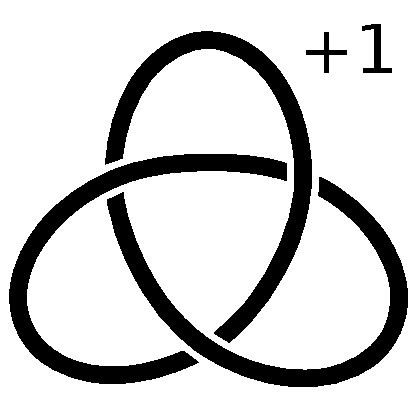
\includegraphics[width=0.5\linewidth]{./pictures/right_handed_trefoil_+1_surgery.pdf}
	\end{center}
	\caption{A Kirby diagram representing the $1$-trace
		$X_1(\textrm{right handed trefoil})$.
		The boundary of this $4$-manifold is the $+1$-surgery
		$\sphere{3}_{+1}(\textrm{right handed trefoil})$,
		a possible description of the Poincar\'e homology sphere.}
	\label{fig:right_handed_trefoil_+1_surgery}
\end{marginfigure}

\begin{theorem}
	\begin{itemize}
		\item $K$ is smoothly slice if and only if $X_{0}(K)$ smoothly embeds in $\sphere{4}$.
		\item Similarly, $K$ is topologically slice if and only if $X_{0}(K)$ topologically
		embeds in $\sphere{4}$.
	\end{itemize}
\end{theorem}


\begin{definition}
	The \textit{tunnel number}\index{knot!tunnel number} $t(K)$ of a knot $K \subset \sphere{3}$ is the minimal number of arcs
	that must be added to the knot (forming a graph with three edges at a vertex) so that
	its complement in $\sphere{3}$ is a handlebody. The same definition is
	valid for links. \\
	The boundary will be a minimal Heegaard splitting of the knot complement
	(The knot complement is a manifold with boundary, so what is the definition
	of a Heegard splitting in that case?).
\end{definition}

\begin{remark}
	Every link has a tunnel number, this can be seen by adding a ``vertical''
	tunnel at every crossing in a link diagram.
	This shows that the tunnel number of a knot is always less than or equal
	to the crossing number, $t(K) \le c(K)$.
\end{remark}

\begin{example}
	\begin{itemize}
		\item The unknot is the only knot with tunnel number 0. (Why?)
		\item The trefoil knot has tunnel number 1.
		\item The figure eight knot has tunnel number 1.
	\end{itemize}
\end{example}



\subsection{Arf invariant}

\begin{theorem}
	The Arf invariant of a knot $K$ is related to the Alexander polynomial by
	\begin{equation*}
		\Arf(K) =
		\begin{cases}
			0 & \textrm{if } \Delta_{K}(-1) \equiv \pm 1 \textrm{ modulo } 8 \\
			1 & \textrm{if } \Delta_{K}(-1) \equiv \pm 3 \textrm{ modulo } 8.
		\end{cases}
	\end{equation*}
\end{theorem}

\begin{remark}
	If $K$ is a slice knot, we know that its determinant
	$| \Delta_{K}(-1) |$ is an odd square integer.
	Thus we have $\Delta_{K}(-1) \equiv \pm 1 \textrm{ modulo } 8$
	\marginnote{$(2k+1)^{2} = 4 k^{2} + 4 k + 1 = 4 \underbrace{k (k+1)}_{\text{even}} + 1
		\equiv 1 \textrm{ modulo } 8$}
	and as such $\Arf(K) = 0$; $\Arf$ is a well defined concordance invariant.
\end{remark}

\section{Concordance}

\begin{definition}
	A \textit{smooth link cobordism} \index{link!cobordism} between the links
	$L_0, L_1 \subset \sphere{3}$
	is a smooth, compact, oriented surface
	$\Sigma$ generically embedded in $\sphere{3} \times \interval$ such that
	$\partial \Sigma = \overline{L_{0}} \coprod L_{1}$,
	where $\partial \Sigma \subset \sphere{3} \times \{0, 1\}$.
\end{definition}

\begin{proposition}
	Linking numbers are concordance invariants.
\end{proposition}

\begin{remark}[The Hopf link is ``the most non-slice link'', \citep{krushkal2015slicing}]
	Any link in $\sphere{3}$ bounds immersed smooth disks
	$\coprod^{n} \disk{2} \looparrowright \disk{4}$.
	%TODO
	TODO
\end{remark}


\begin{definition}[Boundary link]
	\marginnote{It is possible that each component
		of a link bounds a Seifert surface missing the other components,
		but still they do not bound disjoint surfaces.}
	A link $L^{n} \subset \sphere{n+2}$ whose components bound disjoint Seifert surfaces
	is called a \textit{boundary link} \index{link!boundary}.
\end{definition}

\begin{example}
	The untwisted Bing double of any knot is a boundary link.
	%TODO
	TODO Insert definition of Bing double
	TODO Insert picture
	TODO Proof that Bing doubles are boundary links
	(draw the taco shells, need 4 copies of the Seifert surface
	of the knot)
\end{example}

\begin{proposition}[{\citep[5.E.1]{rolfsen2003knots}}]
	If any two components of $L^{1} \subset \sphere{3}$
	have nonzero linking number, then $L$ is \textbf{not}
	a boundary link.
\end{proposition}

\begin{proof}
	Use the definition \ref{def:linking_numbers_via_intersections_with_Seifert_surface} 
	of linking number where you count
	the intersection points of one component with a Seifert surface for the
	other.
\end{proof}

\begin{definition}[{Linking number via intersections with a Seifert surface,
	\citep[5.D.(2)]{rolfsen2003knots}}]
	\label{def:linking_numbers_via_intersections_with_Seifert_surface}
	Let $J$ and $K$ be two disjoint oriented knots (e.g. link components).
	Pick a PL Seifert surface $M^{2}$ for $K$, with
	a bicollar $(N, N^{+}, N^{-})$ of the interior $\mathring{M}$.
	Make $J$ transverse to $M$, i.e. assume after a small
	homotopy of $J$ in $\sphere{3} \setminus K$ that
	$J$ meets $M$ in a finite number of points
	and that at each point $J$ passes locally
	from $N^{+}$ to $N^{-}$ or from $N^{-}$ to $N^{+}$.
	Corresponding to this direction, weight the intersection types
	with $+1$ or $-1$.
	\marginnote{On first sight this seems to depend on the
	choice of Seifert surface $M$.}
	The signed sum of these intersection points is the linking
	number $\lk(J, K) \in \Z$.
\end{definition}

\begin{proposition}[{\citep[5.E.8]{rolfsen2003knots}}]
	If a link $L$ is a boundary link, then each component
	represents an element
	in the second commutator subgroup\sidenote{Also called
		\textit{second derived subgroup} or $G^{(2)}$,
		it is generated by elements of
		the form $[[x,y],[z,w]]$.}
	of the fundamental group of the complement
	of the remaining component(s).
\end{proposition}

\section{Braid groups}

\begin{exercise}
	Show that there is a presentation for the braid groups
	with just two generators.
\end{exercise}

\section{TQFTs - Topological Quantum Field Theories}

%TODO
TODO Write down axioms

\marginnote{A monoidal functor is supposed to preserve the identity
objects for the tensor product. Since the empty set is the identity for the tensor product in the bordism category (given by disjoint union of the bordisms), the TQFT should send this to the identity object for
$\otimes_{R}$, which is just the ground ring $R$.}

\section{Open questions}

\begin{openquestion}
	Is the crossing number of a satellite knot bigger than that of its companion?
\end{openquestion}





% % % % % % % % % % % % % % % % % % % % % % % % %
\chapter{4-manifolds}
% % % % % % % % % % % % % % % % % % % % % % % % %

TODO

%----------------------------------------------------------------------------------------

\backmatter

%----------------------------------------------------------------------------------------
%	BIBLIOGRAPHY
%----------------------------------------------------------------------------------------

\bibliography{mybib} % Use the mybib.bib file for the bibliography

%----------------------------------------------------------------------------------------

\printindex % Print the index at the very end of the document

\end{document}
